% Source PDF page 375 (printed p. 361)
因此，先验约束
\[
 l\le\Prob(X\in A\mid X\in B)\le u
\]
可表示为 $p$ 的线性不等式约束
\[
 l d^{\T}p\le c^{\T}p\le u d^{\T}p.
\]

另有几类先验信息，可表示为非线性凸不等式。例如，$X$ 的熵
\[
 -\sum_{i=1}^np_i\log p_i
\]
是 $p$ 的凹函数，因此可用关于 $p$ 的凸不等式施加熵的下界。如果 $q$ 表示另一个分布，即 $q\succeq0$、$\one^{\T}q=1$，则分布 $q$ 与分布 $p$ 之间的Kullback--Leibler散度为
\[
 \sum_{i=1}^np_i\log(p_i/q_i),
\]
它关于 $p$ 凸，关于 $q$ 也凸，见第90页例3.19。因此，可以将 $p$ 与给定分布 $q$ 之间Kullback--Leibler散度的上界，写成 $p$ 的凸不等式。

下面几段将分布 $p$ 的先验信息表示为 $p\in\mathcal P$。假设 $\mathcal P$ 可由线性等式及凸不等式描述，并将基本约束 $p\succeq0$、$\one^{\T}p=1$ 包含在先验信息 $\mathcal P$ 中。

\subsubsection*{对概率与期望求界}
给定分布的先验信息，例如 $p\in\mathcal P$，便可计算某函数期望或某集合概率的上界或下界。例如，为确定所有满足先验信息 $p\in\mathcal P$ 的分布中 $\E f(X)$ 的下界，可求解凸问题
\[
\begin{array}{ll}
\text{最小化}&\sum_{i=1}^nf(\alpha_i)p_i\\
\text{满足}&p\in\mathcal P.
\end{array}
\]

\subsubsection*{最大似然估计}
可以根据从分布中得到的观测，用最大似然估计来估计 $p$。设观测到 $N$ 个独立样本 $x_1,\ldots,x_N$，用 $k_i$ 表示其中取值为 $\alpha_i$ 的样本个数，则 $k_1+\cdots+k_n=N$，即观测样本总数。对数似然函数为
\[
 l(p)=\sum_{i=1}^nk_i\log p_i,
\]
它关于 $p$ 凹。

% Source PDF page 376 (printed p. 362)
$p$ 的最大似然估计可由求解下列凸问题得到：
\[
\begin{array}{ll}
\text{最大化}&l(p)=\sum_{i=1}^nk_i\log p_i\\
\text{满足}&p\in\mathcal P,
\end{array}
\]
变量为 $p$。

\subsubsection*{最大熵}
与先验假设一致的最大熵分布，可由求解凸问题
\[
\begin{array}{ll}
\text{最小化}&\sum_{i=1}^np_i\log p_i\\
\text{满足}&p\in\mathcal P
\end{array}
\]
得到。支持这一方法的人，将最大熵分布描述为所有符合先验信息的分布中最不作偏向、或最随机的分布。

\subsubsection*{最小Kullback--Leibler散度}
通过求解凸问题
\[
\begin{array}{ll}
\text{最小化}&\sum_{i=1}^np_i\log(p_i/q_i)\\
\text{满足}&p\in\mathcal P,
\end{array}
\]
可在所有符合先验信息的分布中，找出与给定先验分布 $q$ 的Kullback--Leibler散度最小的分布 $p$。注意，当先验分布均匀，即 $q=(1/n)\one$ 时，该问题化为最大熵问题。

\begin{origexample}{7.2}
考虑区间 $[-1,1]$ 内100个等距点 $\alpha_i$ 上的概率分布，施加以下先验假设：
\begin{equation}
\begin{aligned}
 \E X&\in[-0.1,0.1],\\
 \E X^2&\in[0.5,0.6],\\
 \E(3X^3-2X)&\in[-0.3,-0.2],\\
 \Prob(X<0)&\in[0.3,0.4].
\end{aligned}\tag{7.8}
\end{equation}
结合约束 $\one^{\T}p=1$、$p\succeq0$，这些约束描述一个概率分布多面体。

图7.2给出了满足这些约束的最大熵分布，它满足
\[
\begin{aligned}
 \E X&=0.056,\\
 \E X^2&=0.5,\\
 \E(3X^3-2X)&=-0.2,\\
 \Prob(X<0)&=0.4.
\end{aligned}
\]
为说明如何对概率求界，我们计算累计分布 $\Prob(X\le\alpha_i)$ 的上、下界，$i=1,\ldots,100$。对每个 $i$，在所有符合先验假设（7.8）的分布上求解两个线性规划，一个最大化 $\Prob(X\le\alpha_i)$，另一个最小化它。

% Source PDF page 377 (printed p. 363)
\begin{figure}[htbp]\centering
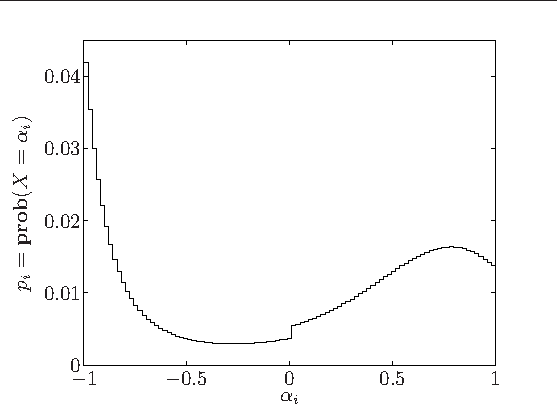
\includegraphics[width=.70\textwidth]{figures/ch07-figure-2.pdf}
\caption*{图7.2\quad 满足约束（7.8）的最大熵分布。}
\end{figure}
结果见图7.3，上、下两条曲线分别为上、下界，中间曲线为最大熵分布的累计分布。
\end{origexample}

\begin{origexample}{7.3}
\textbf{边缘分布已知时风险概率的界。}设随机变量 $X$、$Y$ 表示两项投资的收益。假设 $X$ 取值于 $\{\alpha_1,\ldots,\alpha_n\}\subseteq\R$，$Y$ 取值于 $\{\beta_1,\ldots,\beta_m\}\subseteq\R$，且 $p_{ij}=\Prob(X=\alpha_i,Y=\beta_j)$。两项收益的边缘分布已知，即
\begin{equation}
 \sum_{j=1}^mp_{ij}=r_i,\quad i=1,\ldots,n,\qquad
 \sum_{i=1}^np_{ij}=q_j,\quad j=1,\ldots,m,\tag{7.9}
\end{equation}
但除此以外，对联合分布 $p$ 一无所知。这定义了与给定边缘分布一致的联合分布多面体。

现在同时作这两项投资，总收益为随机变量 $X+Y$。我们希望计算某个损失水平或低收益水平的概率上界，即 $\Prob(X+Y<\gamma)$。求解线性规划
\[
\begin{array}{ll}
\text{最大化}&\sum\{p_{ij}\mid\alpha_i+\beta_j<\gamma\}\\
\text{满足}&\text{（7.9）},\quad p_{ij}\ge0,\quad i=1,\ldots,n,\quad j=1,\ldots,m
\end{array}
\]
可得该概率的紧上界。其最优值是最大的损失概率，最优解 $p^\star$ 是与给定边缘分布一致、且使损失概率最大的联合分布。

同样方法也可用于这两项投资的衍生品。设衍生品收益为 $R(X,Y)$，其中 $R:\R^2\to\R$。

% Source PDF page 378 (printed p. 364)
\begin{figure}[htbp]\centering
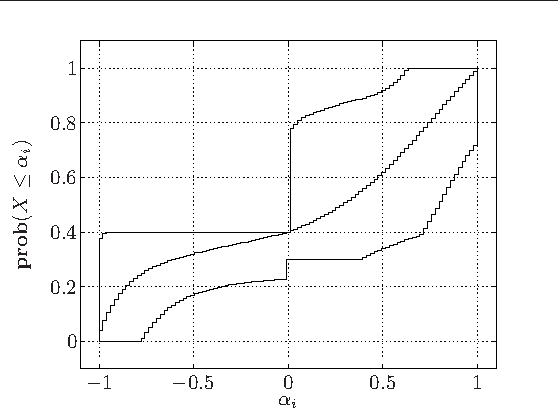
\includegraphics[width=.70\textwidth]{figures/ch07-figure-3.pdf}
\caption*{图7.3\quad 最上方与最下方曲线，表示在所有满足（7.8）的分布中，累计分布函数 $\Prob(X\le\alpha_i)$ 可能达到的最大值与最小值。中间曲线为满足（7.8）的最大熵分布的累计分布。}
\end{figure}
通过求解类似线性规划，对目标函数
\[
 \sum\{p_{ij}\mid R(\alpha_i,\beta_j)<\gamma\}
\]
分别最小化与最大化，就能计算 $\Prob(R<\gamma)$ 的精确下界与上界。
\end{origexample}

\section{最优检测器设计与假设检验}
设随机变量 $X$ 取值于 $\{1,\ldots,n\}$，其分布依赖参数 $\theta\in\{1,\ldots,m\}$。$\theta$ 的 $m$ 种可能取值对应的 $X$ 分布，可用矩阵 $P\in\R^{n\times m}$ 表示，其元素为
\[
 p_{kj}=\Prob(X=k\mid\theta=j).
\]
$P$ 的第 $j$ 列为参数值 $\theta=j$ 对应的概率分布。

考虑根据观测到的一个 $X$ 样本估计 $\theta$。换言之，样本 $X$ 由 $m$ 种可能分布中的一种产生，我们要猜测是哪一种。$\theta$ 的 $m$ 个值称为\emph{假设}，猜测哪个假设正确，即哪个分布生成观测样本 $X$，称为\emph{假设检验}。许多情况下，一个假设对应正常情况，其余各假设分别对应某种异常事件。此时，假设检验可解释为：观测 $X$ 的一个值，然后判断是否发生异常；若发生，又是哪种异常。因此，假设检验也称为\emph{检测}。

% Source PDF page 379 (printed p. 365)
大多数情况下，假设的顺序没有意义，只是任意标记为 $\theta=1,\ldots,m$ 的 $m$ 个不同假设。如果 $\widehat\theta=\theta$，其中 $\widehat\theta$ 是对 $\theta$ 的估计，就正确猜中了参数 $\theta$；如果 $\widehat\theta\ne\theta$，则猜测错误，把 $\widehat\theta$ 误作了 $\theta$。另一些情况下，假设的顺序有意义，这时 $\widehat\theta>\theta$，即高估 $\theta$，就是有意义的事件。

也可以将 $\theta$ 参数化为不属于 $\{1,\ldots,m\}$ 的其他值，例如 $\theta\in\{\theta_1,\ldots,\theta_m\}$，其中 $\theta_i$ 互异。这些值可以是实数，也可以是向量，例如用于指定第 $k$ 个分布的均值与方差。此时，参数估计误差的范数 $\norm{\widehat\theta-\theta}$ 就有意义。

\subsection{确定性检测器与随机化检测器}
确定性\emph{估计器}或\emph{检测器}，是从可能观测值集合 $\{1,\ldots,n\}$ 到假设集合 $\{1,\ldots,m\}$ 的函数 $\psi$。若观测到 $X=k$，就将 $\theta$ 猜为 $\widehat\theta=\psi(k)$。一种显然的确定性检测器是\emph{最大似然检测器}：
\begin{equation}
 \widehat\theta=\psi_{\mathrm{ml}}(k)=\argmax_jp_{kj}.\tag{7.10}
\end{equation}
观测到 $X=k$ 后，$\theta$ 的最大似然估计，就是在可能分布中使观测 $X=k$ 的概率最大的参数值。

我们考虑确定性检测器的一种推广：给定 $X$ 的观测值后，$\theta$ 的估计为随机的。$\theta$ 的\emph{随机化检测器}是一个随机变量 $\widehat\theta\in\{1,\ldots,m\}$，其分布依赖于 $X$ 的观测值。它可由矩阵 $T\in\R^{m\times n}$ 定义，元素为
\[
 t_{ik}=\Prob(\widehat\theta=i\mid X=k).
\]
其含义是：观测到 $X=k$ 时，检测器以概率 $t_{ik}$ 输出 $\widehat\theta=i$。将 $T$ 的第 $k$ 列记为 $t_k$，它给出观测 $X=k$ 时 $\widehat\theta$ 的分布。若 $T$ 每一列都是单位向量，则随机化检测器就是确定性检测器，即 $\widehat\theta$ 是 $X$ 观测值的确定性函数。

乍看起来，在估计或检测过程中故意加入额外随机性，似乎只会使估计器变差。但下面将看到，某些例子中随机化检测器优于所有确定性估计器。

我们关心如何设计定义随机化检测器的矩阵 $T$。显然，$T$ 的各列 $t_k$ 必须满足线性等式与不等式约束
\begin{equation}
 t_k\succeq0,\qquad\one^{\T}t_k=1.\tag{7.11}
\end{equation}

% Source PDF page 380 (printed p. 366)
\subsection{检测概率矩阵}
对矩阵 $T$ 定义的随机化检测器，定义\emph{检测概率矩阵} $D=TP$。有
\[
 D_{ij}=(TP)_{ij}=\Prob(\widehat\theta=i\mid\theta=j),
\]
所以 $D_{ij}$ 表示实际上 $\theta=j$ 时，猜为 $\widehat\theta=i$ 的概率。$m\times m$ 检测概率矩阵 $D$ 刻画了 $T$ 所定义随机化检测器的性能。对角元 $D_{ii}$ 表示 $\theta=i$ 时猜为 $\widehat\theta=i$ 的概率，即正确检测到 $\theta=i$ 的概率。非对角元 $D_{ij}$（$i\ne j$）是将 $\theta=i$ 误作 $\theta=j$ 的概率，也就是实际上 $\theta=j$ 时猜为 $\widehat\theta=i$ 的概率。如果 $D=I$，检测器就是完美的：不论参数 $\theta$ 是什么，都能正确猜为 $\widehat\theta=\theta$。

将 $D$ 的对角元排列成向量，称为\emph{检测概率}，记为 $P^d$：
\[
 P_i^d=D_{ii}=\Prob(\widehat\theta=i\mid\theta=i).
\]
\emph{错误概率}是其补，记为 $P^e$：
\[
 P_i^e=1-D_{ii}=\Prob(\widehat\theta\ne i\mid\theta=i).
\]
由于 $D$ 各列元素之和为一，错误概率也可表示为
\[
 P_i^e=\sum_{j\ne i}D_{ji}.
\]

\subsection{最优检测器设计}
本节说明，检测器设计中的许多目标都是 $D$ 的线性函数、仿射函数或凸分段线性函数，因此也是优化变量 $T$ 的这类函数。类似地，许多约束可用 $D$ 的线性不等式表示。所以，多种最优检测器设计问题都可写成线性规划。第7.3.4节将看到，其中一些问题具有简单解；本节只进行建模。

\subsubsection*{错误与检测概率的限制}
可对正确检测第 $j$ 个假设的概率施加下界：
\[
 P_j^d=D_{jj}\ge L_j,
\]
它是 $D$，从而也是 $T$ 的线性不等式。类似地，可对将 $\theta=i$ 误作 $\theta=j$ 的概率施加上界：
\[
 D_{ij}\le U_{ij}.
\]

% Source PDF page 381 (printed p. 367)
这些同样是 $T$ 的线性约束。任意一个检测概率都可作为待最大化的目标，任意一个错误概率都可作为待最小化的目标。

\subsubsection*{极小极大检测器设计}
可将极小极大错误概率 $\max_jP_j^e$ 作为待最小化目标，它是 $D$，从而也是 $T$ 的分段线性凸函数。只考虑这一目标，得到最小化最大检测错误概率的问题：
\[
\begin{array}{ll}
\text{最小化}&\max_jP_j^e\\
\text{满足}&t_k\succeq0,\quad\one^{\T}t_k=1,\quad k=1,\ldots,n,
\end{array}
\]
变量为 $t_1,\ldots,t_n\in\R^m$。该问题可重写为线性规划。极小极大检测器使 $m$ 个假设中最坏，即最大的错误概率最小。

当然，还可在极小极大检测器设计中加入其他约束。

\subsubsection*{Bayes检测器设计}
Bayes检测器设计给定假设的先验分布 $q\in\R^m$，其中
\[
 q_i=\Prob(\theta=i).
\]
此时，$p_{ij}$ 解释为给定 $\theta$ 时 $X$ 的条件概率。检测器的错误概率为 $q^{\T}P^e$，是 $T$ 的仿射函数。Bayes最优检测器是线性规划
\[
\begin{array}{ll}
\text{最小化}&q^{\T}P^e\\
\text{满足}&t_k\succeq0,\quad\one^{\T}t_k=1,\quad k=1,\ldots,n
\end{array}
\]
的解。第7.3.4节将看到，该问题有简单解析解。

一个特殊情形是 $q=(1/m)\one$，此时Bayes最优检测器最小化各假设的无权平均错误概率。第7.3.4节将说明，最大似然检测器（7.10）对这个问题最优。

\subsubsection*{偏差、均方误差及其他量}
这里假设 $\theta$ 的取值顺序有意义，即当 $i>j$ 时，$\theta=i$ 可理解为比 $\theta=j$ 更大的参数值。例如，若 $\theta=i$ 对应已经发生 $i$ 个事件的假设，就是这种情形。这时可能关心
\[
 \Prob(\widehat\theta>\theta\mid\theta=i),
\]
即 $\theta=i$ 时高估 $\theta$ 的概率。它是 $D$ 的仿射函数：
\[
 \Prob(\widehat\theta>\theta\mid\theta=i)=\sum_{j>i}D_{ji}.
\]

% Source PDF page 382 (printed p. 368)
所以该概率的上限可表示为 $D$，从而也是 $T$ 的线性不等式。再例如，当 $\theta=i$ 时，误判超过一的概率
\[
 \Prob(\abs{\widehat\theta-\theta}>1\mid\theta=i)
 =\sum_{\abs{j-i}>1}D_{ji}
\]
也是 $D$ 的线性函数。

现在设参数取值为 $\{\theta_1,\ldots,\theta_m\}\subseteq\R$。估计或检测的参数误差为 $\widehat\theta-\theta$，若干关心的量都可用 $D$ 的线性函数表示。例如：
\begin{itemize}
\item \emph{偏差。}$\theta=\theta_i$ 时，检测器偏差为线性函数
\[
 \E_i(\widehat\theta-\theta)=\sum_{j=1}^m(\theta_j-\theta_i)D_{ji},
\]
其中 $\E$ 的下标表示，期望是相对于假设 $\theta=\theta_i$ 下的分布计算的。
\item \emph{均方误差。}$\theta=\theta_i$ 时，检测器均方误差为线性函数
\[
 \E_i(\widehat\theta-\theta)^2=\sum_{j=1}^m(\theta_j-\theta_i)^2D_{ji}.
\]
\item \emph{平均绝对误差。}$\theta=\theta_i$ 时，检测器平均绝对误差为线性函数
\[
 \E_i\abs{\widehat\theta-\theta}=\sum_{j=1}^m\abs{\theta_j-\theta_i}D_{ji}.
\]
\end{itemize}

\subsection{多准则形式与标量化}
最优检测器设计可以看作多准则问题，约束为（7.11），$m(m-1)$ 个目标为 $D$ 的非对角元，即不同类型检测错误的概率：
\begin{equation}
\begin{array}{ll}
\text{最小化（关于 }\R_+^{m(m-1)}\text{）}&D_{ij},\quad i,j=1,\ldots,m,\quad i\ne j\\
\text{满足}&t_k\succeq0,\quad\one^{\T}t_k=1,\quad k=1,\ldots,n,
\end{array}\tag{7.12}
\end{equation}
变量为 $t_1,\ldots,t_n\in\R^m$。由于每个目标 $D_{ij}$ 都是变量的线性函数，这是多准则线性规划。

取加权和目标
\[
 \sum_{i,j=1}^mW_{ij}D_{ij}=\tr(W^{\T}D),
\]
可以将其标量化。

% Source PDF page 383 (printed p. 369)
权重矩阵 $W\in\R^{m\times m}$ 满足
\[
 W_{ii}=0,\quad i=1,\ldots,m,\qquad
 W_{ij}>0,\quad i,j=1,\ldots,m,\quad i\ne j.
\]
该目标是 $m(m-1)$ 个错误概率的加权和，$W_{ij}$ 对应实际为 $\theta=j$、却猜为 $\widehat\theta=i$ 的错误。权重矩阵有时称为\emph{损失矩阵}。

为找到多准则问题（7.12）的Pareto最优点，建立标量优化问题
\begin{equation}
\begin{array}{ll}
\text{最小化}&\tr(W^{\T}D)\\
\text{满足}&t_k\succeq0,\quad\one^{\T}t_k=1,\quad k=1,\ldots,n,
\end{array}\tag{7.13}
\end{equation}
它是线性规划，且关于 $t_1,\ldots,t_n$ 可分。目标可写成各 $t_k$ 的线性函数之和：
\[
 \tr(W^{\T}D)=\tr(W^{\T}TP)=\tr(PW^{\T}T)
 =\sum_{k=1}^nc_k^{\T}t_k,
\]
其中 $c_k$ 是 $WP^{\T}$ 的第 $k$ 列。约束也可分，即各 $t_i$ 分别有自己的约束。因此，可以分别求解 $k=1,\ldots,n$ 时的问题
\[
\begin{array}{ll}
\text{最小化}&c_k^{\T}t_k\\
\text{满足}&t_k\succeq0,\quad\one^{\T}t_k=1,
\end{array}
\]
从而求解（7.13）。每个问题都有简单解析解，见习题4.8。先找到索引 $q$，使 $c_{kq}=\min_jc_{kj}$，再取 $t_k^\star=e_q$。这个最优点对应确定性检测器：当观测到 $X=k$ 时，估计为
\begin{equation}
 \widehat\theta=\argmin_j(WP^{\T})_{jk}.\tag{7.14}
\end{equation}
所以，对于非对角元均为正的每个权重矩阵 $W$，都能找到一个使加权和目标最小的确定性检测器。这似乎暗示无需随机化检测器，但下面会看到并非如此。多准则线性规划（7.12）的Pareto最优权衡面为分段线性的；（7.14）形式的确定性检测器，对应Pareto最优面上的顶点。

\subsubsection*{MAP与ML检测器}
考虑先验分布为 $q$ 的Bayes检测器设计。平均错误概率为
\[
 q^{\T}P^e=\sum_{j=1}^mq_j\sum_{i\ne j}D_{ij}
 =\sum_{i,j=1}^mW_{ij}D_{ij},
\]
其中权重矩阵定义为
\[
 W_{ij}=q_j,\quad i,j=1,\ldots,m,\quad i\ne j,\qquad
 W_{ii}=0,\quad i=1,\ldots,m.
\]

% Source PDF page 384 (printed p. 370)
因此，Bayes最优检测器由确定性检测器（7.14）给出，此时
\[
 (WP^{\T})_{jk}=\sum_{i\ne j}q_ip_{ki}
 =\sum_{i=1}^mq_ip_{ki}-q_jp_{kj}.
\]
第一项不依赖 $j$，所以观测到 $X=k$ 时，最优检测器就是
\[
 \widehat\theta=\argmax_j(p_{kj}q_j).
\]
这个解有简单解释：$p_{kj}q_j$ 是 $\theta=j$ 且 $X=k$ 的概率，因此该检测器为\emph{最大后验概率}（MAP）检测器。

特别地，若 $q=(1/m)\one$，即 $\theta$ 的先验分布均匀，该MAP检测器化为\emph{最大似然}（ML）检测器：
\[
 \widehat\theta=\argmax_jp_{kj}.
\]
所以，最大似然检测器最小化无权平均错误概率。

\subsection{二元假设检验}
作为说明，考虑 $m=2$ 的特殊情形，称为\emph{二元假设检验}。随机变量 $X$ 由两个分布中的一个产生，为简化记号，将两个分布记为 $p\in\R^n$、$q\in\R^n$。通常，$\theta=1$ 对应正常情况，$\theta=2$ 对应要检测的某种异常事件。若 $\widehat\theta=1$，称检验为\emph{阴性}，即猜测事件未发生；若 $\widehat\theta=2$，称为\emph{阳性}，即猜测事件已发生。

检测概率矩阵 $D\in\R^{2\times2}$ 通常写成
\[
 D=\begin{bmatrix}1-P_{\mathrm{fp}}&P_{\mathrm{fn}}\\
 P_{\mathrm{fp}}&1-P_{\mathrm{fn}}\end{bmatrix}.
\]
$P_{\mathrm{fn}}$ 是\emph{假阴性}概率，即事件实际发生但检验为阴性；$P_{\mathrm{fp}}$ 是\emph{假阳性}概率，即事件实际未发生但检验为阳性，也称为\emph{虚警概率}。最优检测器设计是以 $P_{\mathrm{fn}}$、$P_{\mathrm{fp}}$ 为目标的双准则问题。

两者的最优权衡曲线称为\emph{接收者工作特征}（ROC），由分布 $p,q$ 确定。按照第7.3.4节对双准则问题进行标量化，便可求出ROC。给定权重矩阵 $W$，最优检测器（7.14）为
\[
 \widehat\theta=\begin{cases}
 1&W_{21}p_k>W_{12}q_k,\\
 2&W_{21}p_k\le W_{12}q_k.
 \end{cases}
\]
